\documentclass[12pt, twoside]{article}
\usepackage[letterpaper, margin=1in, headsep=0.5in]{geometry}
\usepackage[english]{babel}
\usepackage[utf8]{inputenc}
\usepackage{amsmath}
\usepackage{amsfonts}
\usepackage{amssymb}
\usepackage{tikz}
%\usetikzlibrary{quotes, angles}

\usepackage{graphicx}
\usepackage{enumitem}
\usepackage{multicol}

\usepackage{fancyhdr}
\pagestyle{fancy}
\fancyhf{}
\renewcommand{\headrulewidth}{0pt} % disable the underline of the header

\fancyhead[RE]{\thepage}
\fancyhead[RO]{\thepage \\ Name: \hspace{3cm}}
\fancyhead[L]{BECA / Dr. Huson / 10th Grade Geometry\\* 17 December 2018}

\begin{document}
\subsubsection*{Homework: Transformations practice (due Tuesday)}
 \begin{enumerate}

  \begin{multicols}{2}
    [\item A translation maps triangle $ABC$ onto triangle $DEF$.] \vspace{0.5cm}
      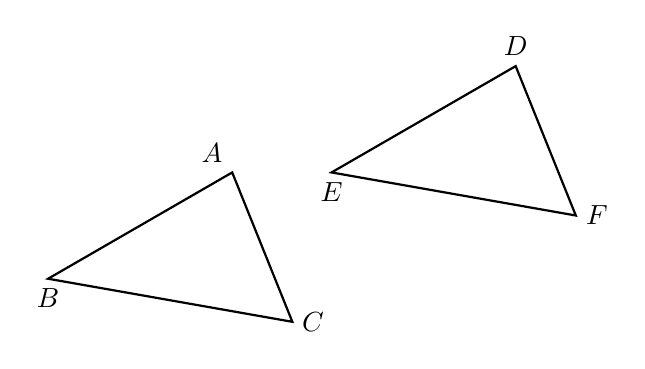
\begin{tikzpicture}[scale=0.9]
        \coordinate [label=above left:$A$](A) at (30:3);
        \coordinate [label=below:$B$](B) at (0, 0);
        \coordinate [label=right:$C$](C) at (-10:3.5);
        \draw [thick] (A)--(B)--(C)--cycle;

        \draw [thick, xshift=4cm, yshift=1.5cm] (30:3) node[above]{$D$}--
        (0,0) node[below]{$E$}--
        (-10:3.5) node[right]{$F$}--cycle;
      \end{tikzpicture}\\
      Fill in the blank with the corresponding object.
      \begin{enumerate}
        \item $A \rightarrow$ \rule{2cm}{0.15mm} \vspace{0.3cm}
        \item $\angle ABC \cong$ \rule{2cm}{0.15mm}
        \item \rule{2cm}{0.15mm} $\cong \overline {EF}$
      \end{enumerate}
    \end{multicols} \vspace{1cm}

   \item The vertices of $\triangle JKL$ have the coordinates $J(-4,-2)$, $K(-1,-1)$, and $L(-2,3)$, as shown below. \\[0.5cm]
   Apply a translation of $(x,y) \rightarrow (x+7, y+4)$ to $\triangle JKL$ and then reflect the image across the $x$-axis. Draw both images $\triangle J'K'L'$ and $\triangle J''K''L''$ on the set of axes below, labeling the vertices.
   \begin{center}
     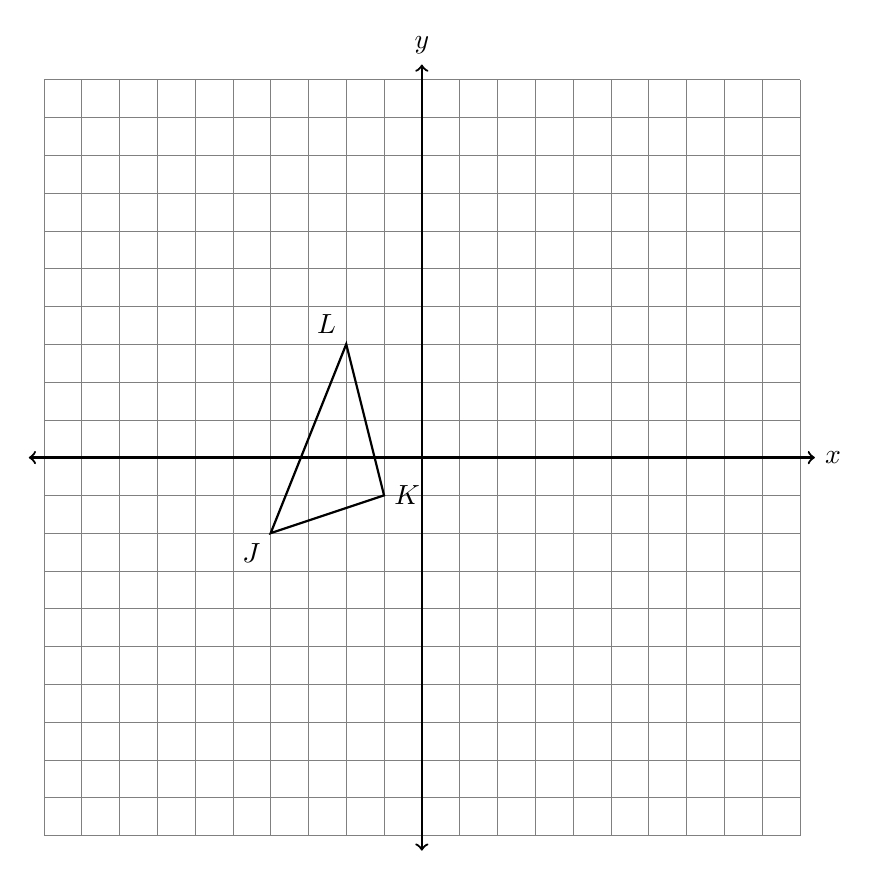
\begin{tikzpicture}[scale=.48]
       \draw [help lines] (-10,-10) grid (10,10);
       \draw [thick, <->] (-10.4,0) -- (10.4,0) node [right] {$x$};
       \draw [thick, <->] (0,-10.4)--(0,10.4) node [above] {$y$};

       \draw [thick]
       (-4,-2) node[below left] {$J$}--
       (-1,-1) node[right] {$K$}--
       (-2,3) node[above left] {$L$}--
       cycle;
     \end{tikzpicture}\\[0.5cm]
\end{center}

\newpage
\item A rotation of $90^\circ$ is applied to $\triangle ABC$, mapping it onto $\triangle PQR$, as shown.  \\[0.25cm]
Which triangle has the larger area, or are they equal? Justify your answer.\\
    \begin{tikzpicture}[scale=.48]
      \draw [thick, <->] (-7.4,0) -- (10.4,0) node [right] {$x$};
      \draw [thick, <->] (0,-6.4)--(0,10.4) node [above] {$y$};

      \draw [thick]
      (4,-2) node[below left] {$A$}--
      (8,2) node[right] {$B$}--
      (1,1) node[above right] {$C$}--cycle;

      \draw [thick]
      (2,4) node[right] {$P$}--
      (-2,8) node[above] {$Q$}--
      (-1,1) node[below left] {$R$}--cycle;

    \end{tikzpicture}

\item The trapezoid $MATH$, shown below, undergoes two rigid motions carrying it onto trapezoid $COMP$. State the two isometric transformations. (there is more than one correct answer)\\
  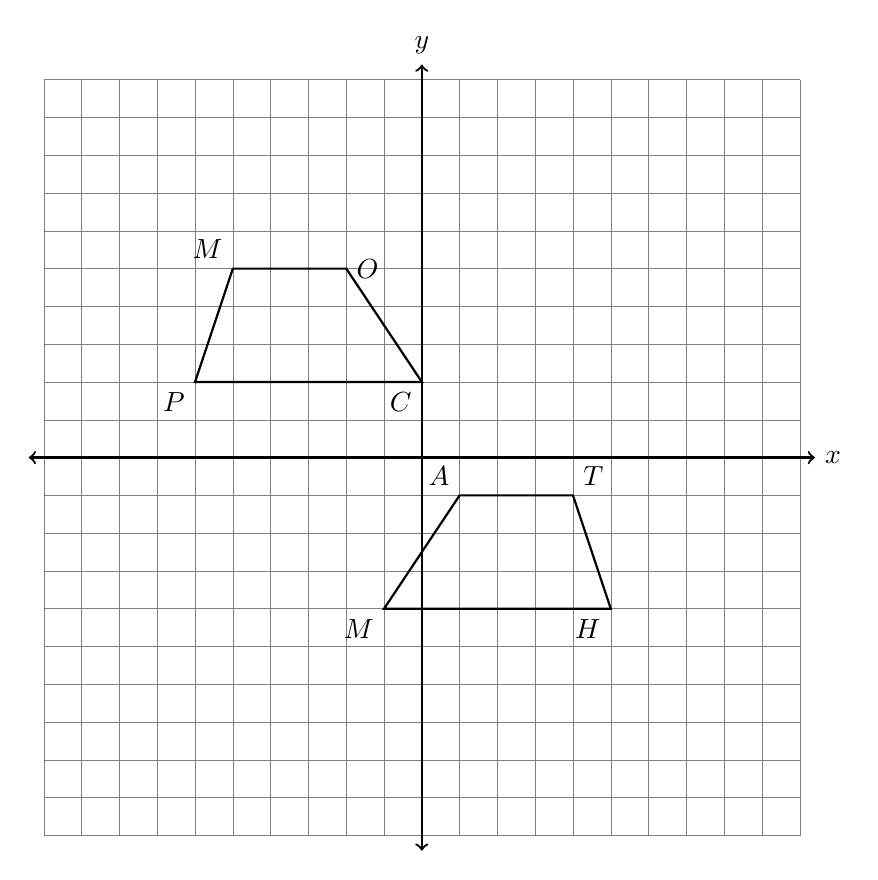
\begin{tikzpicture}[scale=.48]
    \draw [help lines] (-10,-10) grid (10,10);
    \draw [thick, <->] (-10.4,0) -- (10.4,0) node [right] {$x$};
    \draw [thick, <->] (0,-10.4)--(0,10.4) node [above] {$y$};

    \draw [thick]
    (-1,-4) node[below left] {$M$}--
    (1,-1) node[above left] {$A$}--
    (4,-1) node[above right] {$T$}--
    (5,-4) node[below left] {$H$}--cycle;

    \draw [thick]
    (0,2) node[below left] {$C$}--
    (-2,5) node[right] {$O$}--
    (-5,5) node[above left] {$M$}--
    (-6,2) node[below left] {$P$}--cycle;

  \end{tikzpicture}

\end{enumerate}
\end{document}
